\documentclass[11pt]{article}

\usepackage{exscale}
\usepackage{graphicx}
\usepackage{amsmath}
\usepackage{amsthm}
\usepackage{latexsym}
\usepackage{times,mathptm}
\usepackage{epsfig}
\usepackage{amssymb}
\usepackage{tikz}

\textwidth 6.5truein          
\textheight 9.0truein
\oddsidemargin 0.0in
\topmargin -0.6in

\parindent 0pt          
\parskip 5pt
\def\baselinestretch{1.1}

\begin{document}

\begin{LARGE}
\centerline {\bf CSci 423 Homework 1}
\end{LARGE}
\vskip 0.25cm

\centerline{Due: 9:30 am, Thursday, 9/10}
\centerline{Alexander Powell}


\begin{enumerate}

\item (10 points) Prove by induction that $\sum_{i=1}^n i^3 = (\sum_{i=1}^n i)^2$.

\begin{proof}

Base Step: When $n = 1$, then we have that $\sum_{i=1}^1 i^3 = 1^3 = 1$ and $(\sum_{i=1}^1 i)^2 = 1^2 = 1$.  Because the left side equals the right side when $i=1$ the base step is true.  

Now suppose it is true for $n=k$.  Making the inductive step, we have that 
$$ \sum_{i=1}^{k+1} i^3 = \sum_{i=1}^k i^3 + (k+1)^3 = \bigg(\sum_{i=1}^k i\bigg)^2 + (k+1)^3 $$
Using the well known series: $$\sum_{k=1}^n k = \frac{n(n+1)}{2},$$ we can rewrite the previous expression to be 
$$ \bigg(\frac{k(k+1)}{2}\bigg)^2 + (k+1)^3 = \frac{k^2(k+1)^2}{4} + k^3 + 3k^2 + 3k + 1 $$
$$ = \frac{(k^2)(k^2+2k+1)}{4} + k^3 + 3k^2 + 3k + 1 $$
$$ = \frac{k^4+2k^3+k^2}{4} + k^3 + 3k^2 + 3k + 1 = \frac{k^4 + 6k^3 + 13k^2 + 12k + 4}{4} $$
$$ = \frac{(k+1)^2(k+2)^2}{(2)^2} = \bigg( \frac{(k+1)((k+1)+1)}{2} \bigg)^2 = \bigg( \sum_{i=1}^{k+1} \bigg)^2. $$

Thus, we have proven by induction that $\sum_{i=1}^n i^3 = (\sum_{i=1}^n i)^2$.

\end{proof}
Collaborators:

\item (5 points) Prove by contradiction that $\sqrt{3}$ is not a rational number.

\begin{proof}

Assume that $\sqrt{3}$ is a rational number.  Then we can also state that $\sqrt{3} = \frac{m}{n}, m,n \in \mathbb{Z}$ and $\gcd(m,n) = 1$.  With a little manipulation we can write $3 = \frac{m^2}{n^2}$ so $m^2 = 3n^2$.  From here there are two cases: $n$ can be even or $n$ can be odd.  

If $n$ is even then $m$ is also even and therefore the $\gcd(m,n) \neq 1$, which is a contradiction to our original assumption.  

If $n$ is odd then $m$ is also odd so we can write 
$$m = 2a+1, n = 2b+1, a,b \in \mathbb{Z}.$$
With a little algebra we get 
$$ (2a+1)^2 = 3(2b+1)^2 $$
$$ (4a^2+4a+1) = 3(4b^2+4b+1)^2 $$
$$ 4a^2 + 4a + 1 = 12b^2 + 12b + 3 $$
$$ 2a^2 + 2a = 6b^2 + 6b + 1 $$
$$ 2(a^2 + a) = 2(3b^2 + 3b) + 1 $$
Since the left-hand side of the equation is even (some number multiplied by $2$) and the right-hand side is odd (some number mulitplied by $2$ and then add $1$) we arrive at another contradiction.  

Therefore, the original statement holds and thus the $\sqrt{3}$ is an irrational number.  

\end{proof}
Collaborators:

\item (9 points) Give the state diagram of a DFA (with 15 states) that recognizes the set of strings such that in each string the number of 0s is divisible by 5 and the number of 1s is divisible by 3.

The following DFA accepts all strings on the given alphabet where the number of 0s is divisible by 5 and the number of 1s is divisible by 3.  This works because once a 0 has been added, 4 more must be added before the 'loop' is complete, and similarly with 1s.  Note that there is only one start state and end state and they are the same state.  Also, this DFA assumes that 0 is divisible by both 5 and 3, for cases where the string has either no 0s or no 1s.  

%\iffalse
\begin{center}
\begin{tikzpicture}[scale=0.2]
\tikzstyle{every node}+=[inner sep=0pt]
\draw [black] (20.9,-5) circle (3);
\draw (20.9,-5) node {$q_0$};
\draw [black] (20.9,-5) circle (2.4);
\draw [black] (39.2,-5) circle (3);
\draw (39.2,-5) node {$q_1$};
\draw [black] (57.5,-5) circle (3);
\draw (57.5,-5) node {$q_2$};
\draw [black] (20.9,-17.1) circle (3);
\draw (20.9,-17.1) node {$q_3$};
\draw [black] (39.2,-17.1) circle (3);
\draw (39.2,-17.1) node {$q_4$};
\draw [black] (57.5,-17.1) circle (3);
\draw (57.5,-17.1) node {$q_5$};
\draw [black] (20.9,-29.2) circle (3);
\draw (20.9,-29.2) node {$q_6$};
\draw [black] (39.2,-29.2) circle (3);
\draw (39.2,-29.2) node {$q_7$};
\draw [black] (57.5,-29.2) circle (3);
\draw (57.5,-29.2) node {$q_8$};
\draw [black] (20.9,-40.8) circle (3);
\draw (20.9,-40.8) node {$q_9$};
\draw [black] (39.2,-40.8) circle (3);
\draw (39.2,-40.8) node {$q_1_0$};
\draw [black] (57.5,-40.8) circle (3);
\draw (57.5,-40.8) node {$q_1_1$};
\draw [black] (20.9,-52.1) circle (3);
\draw (20.9,-52.1) node {$q_1_2$};
\draw [black] (39.2,-52.1) circle (3);
\draw (39.2,-52.1) node {$q_1_3$};
\draw [black] (57.5,-52.1) circle (3);
\draw (57.5,-52.1) node {$q_1_4$};
\draw [black] (14.3,-1.9) -- (18.18,-3.72);
\fill [black] (18.18,-3.72) -- (17.67,-2.93) -- (17.25,-3.84);
\draw [black] (20.9,-8) -- (20.9,-14.1);
\fill [black] (20.9,-14.1) -- (21.4,-13.3) -- (20.4,-13.3);
\draw (20.4,-11.05) node [left] {$0$};
\draw [black] (20.9,-32.2) -- (20.9,-37.8);
\fill [black] (20.9,-37.8) -- (21.4,-37) -- (20.4,-37);
\draw (20.4,-35) node [left] {$0$};
\draw [black] (20.9,-43.8) -- (20.9,-49.1);
\fill [black] (20.9,-49.1) -- (21.4,-48.3) -- (20.4,-48.3);
\draw (20.4,-46.45) node [left] {$0$};
\draw [black] (39.2,-8) -- (39.2,-14.1);
\fill [black] (39.2,-14.1) -- (39.7,-13.3) -- (38.7,-13.3);
\draw (39.7,-11.05) node [right] {$0$};
\draw [black] (39.2,-32.2) -- (39.2,-37.8);
\fill [black] (39.2,-37.8) -- (39.7,-37) -- (38.7,-37);
\draw (39.7,-35) node [right] {$0$};
\draw [black] (39.2,-43.8) -- (39.2,-49.1);
\fill [black] (39.2,-49.1) -- (39.7,-48.3) -- (38.7,-48.3);
\draw (39.7,-46.45) node [right] {$0$};
\draw [black] (57.5,-8) -- (57.5,-14.1);
\fill [black] (57.5,-14.1) -- (58,-13.3) -- (57,-13.3);
\draw (57,-11.05) node [left] {$0$};
\draw [black] (57.5,-20.1) -- (57.5,-26.2);
\fill [black] (57.5,-26.2) -- (58,-25.4) -- (57,-25.4);
\draw (57,-23.15) node [left] {$0$};
\draw [black] (57.5,-32.2) -- (57.5,-37.8);
\fill [black] (57.5,-37.8) -- (58,-37) -- (57,-37);
\draw (57,-35) node [left] {$0$};
\draw [black] (57.5,-43.8) -- (57.5,-49.1);
\fill [black] (57.5,-49.1) -- (58,-48.3) -- (57,-48.3);
\draw (57,-46.45) node [left] {$0$};
\draw [black] (54.87,-6.442) arc (-63.68886:-116.31114:35.354);
\fill [black] (23.53,-6.44) -- (24.03,-7.24) -- (24.47,-6.35);
\draw (39.2,-10.6) node [below] {$\mbox{ }\mbox{ }\mbox{ }\mbox{ }\mbox{ }\mbox{ }\mbox{ }\mbox{ }\mbox{ }\mbox{ }\mbox{ }\mbox{ }\mbox{ }\mbox{ }\mbox{ }\mbox{ }\mbox{ }\mbox{ }\mbox{ }\mbox{ }\mbox{ }\mbox{ }\mbox{ }\mbox{ }\mbox{ }\mbox{ }\mbox{ }\mbox{ }\mbox{ }\mbox{ }\mbox{ }\mbox{ }\mbox{ }1$};
\draw [black] (54.794,-18.393) arc (-66.65439:-113.34561:39.35);
\fill [black] (23.61,-18.39) -- (24.14,-19.17) -- (24.54,-18.25);
\draw (39.2,-22.11) node [below] {$\mbox{ }\mbox{ }\mbox{ }\mbox{ }\mbox{ }\mbox{ }\mbox{ }\mbox{ }\mbox{ }\mbox{ }\mbox{ }\mbox{ }\mbox{ }\mbox{ }\mbox{ }\mbox{ }\mbox{ }\mbox{ }\mbox{ }\mbox{ }\mbox{ }\mbox{ }1$};
\draw [black] (54.875,-30.651) arc (-63.51339:-116.48661:35.147);
\fill [black] (23.52,-30.65) -- (24.02,-31.46) -- (24.46,-30.56);
\draw (39.2,-34.84) node [below] {$\mbox{ }\mbox{ }\mbox{ }\mbox{ }\mbox{ }\mbox{ }\mbox{ }\mbox{ }\mbox{ }\mbox{ }\mbox{ }\mbox{ }\mbox{ }\mbox{ }\mbox{ }\mbox{ }\mbox{ }\mbox{ }\mbox{ }\mbox{ }\mbox{ }1$};
\draw [black] (54.81,-42.126) arc (-66.00962:-113.99038:38.392);
\fill [black] (23.59,-42.13) -- (24.12,-42.91) -- (24.52,-41.99);
\draw (39.2,-45.94) node [below] {$\mbox{ }\mbox{ }\mbox{ }\mbox{ }\mbox{ }\mbox{ }\mbox{ }\mbox{ }\mbox{ }\mbox{ }\mbox{ }\mbox{ }\mbox{ }\mbox{ }\mbox{ }\mbox{ }\mbox{ }\mbox{ }\mbox{ }\mbox{ }\mbox{ }\mbox{ }\mbox{ }\mbox{ }\mbox{ }1$};
\draw [black] (54.856,-53.516) arc (-64.20678:-115.79322:35.981);
\fill [black] (23.54,-53.52) -- (24.05,-54.31) -- (24.48,-53.41);
\draw (39.2,-57.6) node [below] {$\mbox{ }\mbox{ }\mbox{ }\mbox{ }\mbox{ }\mbox{ }\mbox{ }\mbox{ }\mbox{ }\mbox{ }\mbox{ }\mbox{ }\mbox{ }\mbox{ }\mbox{ }\mbox{ }\mbox{ }\mbox{ }\mbox{ }\mbox{ }\mbox{ }\mbox{ }\mbox{ }1$};
\draw [black] (23.9,-52.1) -- (36.2,-52.1);
\fill [black] (36.2,-52.1) -- (35.4,-51.6) -- (35.4,-52.6);
\draw (30.05,-52.6) node [below] {$1$};
\draw [black] (42.2,-52.1) -- (54.5,-52.1);
\fill [black] (54.5,-52.1) -- (53.7,-51.6) -- (53.7,-52.6);
\draw (48.35,-52.6) node [below] {$1$};
\draw [black] (23.9,-40.8) -- (36.2,-40.8);
\fill [black] (36.2,-40.8) -- (35.4,-40.3) -- (35.4,-41.3);
\draw (30.05,-41.3) node [below] {$1$};
\draw [black] (23.9,-29.2) -- (36.2,-29.2);
\fill [black] (36.2,-29.2) -- (35.4,-28.7) -- (35.4,-29.7);
\draw (30.05,-29.7) node [below] {$1$};
\draw [black] (23.9,-17.1) -- (36.2,-17.1);
\fill [black] (36.2,-17.1) -- (35.4,-16.6) -- (35.4,-17.6);
\draw (30.05,-17.6) node [below] {$1$};
\draw [black] (23.9,-5) -- (36.2,-5);
\fill [black] (36.2,-5) -- (35.4,-4.5) -- (35.4,-5.5);
\draw (30.05,-5.5) node [below] {$1$};
\draw [black] (42.2,-5) -- (54.5,-5);
\fill [black] (54.5,-5) -- (53.7,-4.5) -- (53.7,-5.5);
\draw (48.35,-5.5) node [below] {$1$};
\draw [black] (42.2,-17.1) -- (54.5,-17.1);
\fill [black] (54.5,-17.1) -- (53.7,-16.6) -- (53.7,-17.6);
\draw (48.35,-17.6) node [below] {$1$};
\draw [black] (42.2,-29.2) -- (54.5,-29.2);
\fill [black] (54.5,-29.2) -- (53.7,-28.7) -- (53.7,-29.7);
\draw (48.35,-29.7) node [below] {$1$};
\draw [black] (42.2,-40.8) -- (54.5,-40.8);
\fill [black] (54.5,-40.8) -- (53.7,-40.3) -- (53.7,-41.3);
\draw (48.35,-41.3) node [below] {$1$};
\draw [black] (19.119,-49.687) arc (-145.85227:-214.14773:37.655);
\fill [black] (19.12,-7.41) -- (18.26,-7.79) -- (19.08,-8.36);
\draw (12.13,-28.55) node [left] {$0$};
\draw [black] (37.932,-49.382) arc (-156.62557:-203.37443:52.507);
\fill [black] (37.93,-7.72) -- (37.16,-8.25) -- (38.07,-8.65);
\draw (33.12,-28.55) node [left] {$0$};
\draw [black] (20.9,-20.1) -- (20.9,-26.2);
\fill [black] (20.9,-26.2) -- (21.4,-25.4) -- (20.4,-25.4);
\draw (20.4,-23.15) node [left] {$0$};
\draw [black] (39.2,-20.1) -- (39.2,-26.2);
\fill [black] (39.2,-26.2) -- (39.7,-25.4) -- (38.7,-25.4);
\draw (39.7,-23.15) node [right] {$0$};
\draw [black] (59.57,-7.17) arc (41.00787:-41.00787:32.583);
\fill [black] (59.57,-7.17) -- (59.72,-8.1) -- (60.47,-7.45);
\draw (68.07,-28.55) node [right] {$0$};
\end{tikzpicture}
\end{center}
%\fi
Collaborators: Derek O'connell

\item (6 points) Give the state diagram of a DFA (with 3 states) that accepts all strings on alphabet $\{0,1\}$, except for those strings containing substring 001.

The DFA below accepts all strings on the given alphabet except those containing the substring 001.  Note that for this to work every state has to be an endstate for cases when the length of a string is less than $3$.  

\begin{center}
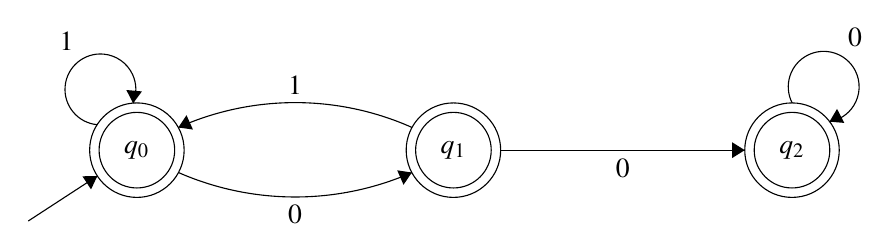
\begin{tikzpicture}[scale=0.2]
\tikzstyle{every node}+=[inner sep=0pt]
\draw [black] (15.7,-9.7) circle (3);
\draw (15.7,-9.7) node {$q_0$};
\draw [black] (15.7,-9.7) circle (2.4);
\draw [black] (35.8,-9.7) circle (3);
\draw (35.8,-9.7) node {$q_1$};
\draw [black] (35.8,-9.7) circle (2.4);
\draw [black] (57.3,-9.7) circle (3);
\draw (57.3,-9.7) node {$q_2$};
\draw [black] (57.3,-9.7) circle (2.4);
\draw [black] (8.8,-14.2) -- (13.19,-11.34);
\fill [black] (13.19,-11.34) -- (12.24,-11.36) -- (12.79,-12.19);
\draw [black] (13.187,-8.083) arc (264.96376:-23.03624:2.25);
\draw (11.23,-3.41) node [above] {$1$};
\fill [black] (15.46,-6.72) -- (16.02,-5.97) -- (15.03,-5.88);
\draw [black] (33.162,-11.121) arc (-66.33938:-113.66062:18.469);
\fill [black] (33.16,-11.12) -- (32.23,-10.98) -- (32.63,-11.9);
\draw (25.75,-13.17) node [below] {$0$};
\draw [black] (38.8,-9.7) -- (54.3,-9.7);
\fill [black] (54.3,-9.7) -- (53.5,-9.2) -- (53.5,-10.2);
\draw (46.55,-10.2) node [below] {$0$};
\draw [black] (18.328,-8.259) arc (114.02176:65.97824:18.233);
\fill [black] (18.33,-8.26) -- (19.26,-8.39) -- (18.85,-7.48);
\draw (25.75,-6.18) node [above] {$1$};
\draw [black] (57.316,-6.712) arc (207.43495:-80.56505:2.25);
\draw (61.31,-3.16) node [above] {$0$};
\fill [black] (59.68,-7.89) -- (60.62,-7.97) -- (60.16,-7.08);
\end{tikzpicture}
\end{center}

Collaborators: Derek O'connell

\end{enumerate}

\end{document}